% Open-Ended Lab report, IEEE conference format. Build with build.ps1 in this folder; it writes OEL-Report.pdf.
\documentclass[conference,a4paper]{IEEEtran}

% Times for the text, as IEEE papers are set, and a monospaced face for code and commands. Tectonic's engine is XeTeX,
% so the fonts are named by file, from its bundle, rather than looked up on the system.
\usepackage{fontspec}
\setmainfont{texgyretermes}[Extension=.otf, UprightFont=*-regular, BoldFont=*-bold, ItalicFont=*-italic,
  BoldItalicFont=*-bolditalic, Ligatures=TeX]
\setmonofont{DejaVuSansMono}[Extension=.ttf, BoldFont=*-Bold, ItalicFont=*-Oblique, BoldItalicFont=*-BoldOblique,
  Scale=0.82]

\usepackage{cite}
\usepackage{graphicx}
\usepackage{xcolor}
\usepackage{listings}
\usepackage{booktabs}
\usepackage{tabularx}
\usepackage{array}
\usepackage{tikz}
\usetikzlibrary{positioning,arrows.meta}
\usepackage{microtype}
\usepackage{url}
\usepackage[hidelinks]{hyperref}

% table columns that wrap ragged-right: L{width}, and Y taking what is left in a tabularx
\newcolumntype{L}[1]{>{\raggedright\arraybackslash}p{#1}}
\newcolumntype{Y}{>{\raggedright\arraybackslash}X}

% ---------------------------------------------------------------------------------------------------------------
% Unfinished text. \gap{...} prints in red; build.ps1 counts what is left, and -Final refuses to build while any is.
% ---------------------------------------------------------------------------------------------------------------
\definecolor{gap}{RGB}{200,0,0}
\newcommand{\gap}[1]{\leavevmode{\color{gap}\textbf{[}\textit{#1}\textbf{]}}}

% Who wrote the report, for whom, and when. The only file to edit for the title block.
% A value still wrapped in \gap{...} prints in red and is counted by build.ps1 as unfinished.
%
% Sources: the course code, department and semester are from the cover of the course's lab manual ("Software
% Construction (SE-314), Fall Semester, Department of Computer Software Engineering"); the lab engineer is the one
% the lab tasks are submitted to ("LE Aqsa", Lab Task 8, 20 November 2026).
\newcommand{\MemberOneName}{Hamza Rasool}
\newcommand{\MemberOneReg}{534756}

\newcommand{\MemberTwoName}{Abdullah Khan}
\newcommand{\MemberTwoReg}{514657}

\newcommand{\LabEngineer}{Aqsa}

\newcommand{\Course}{Software Construction}
\newcommand{\CourseCode}{SE-314}
\newcommand{\Semester}{Fall 2026}
\newcommand{\Class}{BESE-30}
\newcommand{\Department}{Department of Computer Software Engineering}
\newcommand{\Institution}{Military College of Signals\\NUST}
\newcommand{\SubmissionDate}{22 November 2026}

\newcommand{\RepoURL}{\url{https://github.com/hamdotexe/taskmanager}}


% The commit table and its counts, written by build.ps1 from git log at every build
\InputIfFileExists{generated/history}{}{}
\providecommand{\CommitCount}{\gap{number}}
\providecommand{\FirstCommitDate}{\gap{date}}
\providecommand{\LastCommitDate}{\gap{date}}
\providecommand{\CommitRows}{\multicolumn{4}{l}{\gap{git log was not available to build.ps1}}\\}

% ---------------------------------------------------------------------------------------------------------------
% Screenshots. \screenshot{name}{caption}{what it must show} sits in one column, \screenshotwide{...} spans both.
% Each includes screenshots/<name>.png when the file is there, and otherwise draws a framed placeholder naming it,
% so the report builds at every stage.
% ---------------------------------------------------------------------------------------------------------------
\newcommand{\shotpath}[1]{screenshots/#1.png}
\newcommand{\shotplaceholder}[3]{{%
  \color{gap}\setlength{\fboxsep}{6pt}%
  \fbox{\parbox[c][#3][c]{\dimexpr\linewidth-2\fboxsep-2\fboxrule\relax}{\centering\footnotesize
    \textbf{Screenshot not yet taken}\\[3pt]
    \texttt{report/screenshots/#1.png}\\[3pt]
    \textit{#2}}}}}
% \shotimage{name}{what it must show}{largest height}{placeholder height}
\newcommand{\shotimage}[4]{%
  \IfFileExists{\shotpath{#1}}%
    {\includegraphics[width=\linewidth,height=#3,keepaspectratio]{\shotpath{#1}}}%
    {\shotplaceholder{#1}{#2}{#4}}}
% A placeholder is about as tall as the screenshot will be, so the layout of a draft is close to the final one.
\newcommand{\screenshot}[3]{%
  \begin{figure}[!tbp]
    \centering
    \shotimage{#1}{#3}{0.4\textheight}{5cm}
    \caption{#2}\label{fig:#1}
  \end{figure}}
\newcommand{\screenshotwide}[3]{%
  \begin{figure*}[!tp]
    \centering
    \shotimage{#1}{#3}{0.45\textheight}{9.5cm}
    \caption{#2}\label{fig:#1}
  \end{figure*}}

% Let a page take two wide figures at its top, and two of them make a page of their own, so that the many wide
% screenshots do not queue up and drift away from the text they belong to.
\renewcommand{\topfraction}{0.9}
\renewcommand{\dbltopfraction}{0.9}
\renewcommand{\textfraction}{0.07}
\renewcommand{\floatpagefraction}{0.6}
\renewcommand{\dblfloatpagefraction}{0.6}
\setcounter{topnumber}{3}
\setcounter{dbltopnumber}{2}
\setcounter{totalnumber}{4}

% ---------------------------------------------------------------------------------------------------------------
% Listings. Transcripts are quoted as they are from ../../evidence (outside the repository); source code is quoted
% from the repository's own files, so a quote can never drift from the code it shows.
% ---------------------------------------------------------------------------------------------------------------
\newcommand{\evidencedir}{../../evidence}
\newcommand{\srcdir}{..}
\lstdefinestyle{terminal}{
  basicstyle=\ttfamily\scriptsize, columns=fixed, keepspaces=true, upquote=true, tabsize=8,
  breaklines=true, postbreak=\mbox{\textcolor{gray}{$\hookrightarrow$}\space},
  frame=tb, framesep=3pt, aboveskip=6pt, belowskip=6pt, captionpos=t, abovecaptionskip=0pt, belowcaptionskip=5pt,
  showstringspaces=false}
% IEEEtran's caption leaves out the space below it that listings asks for, so the caption sat on the listing's rule
\makeatletter
\def\lst@makecaption#1#2{\vskip\abovecaptionskip\@makecaption{#1}{#2}\par\vskip\belowcaptionskip}
\makeatother
\lstdefinestyle{java}{
  style=terminal, language=Java, keywordstyle=\bfseries, commentstyle=\color{black!60}\itshape,
  morekeywords={record,var}}
% \evidence[listing options]{file}{caption}
\newcommand{\evidence}[3][]{%
  \IfFileExists{\evidencedir/#2}%
    {\lstinputlisting[style=terminal,caption={#3},label={lst:#2},#1]{\evidencedir/#2}}%
    {\par\gap{Transcript evidence/#2 not found}\par}}
% \source[listing options]{path in the repository}{caption}{label}: kept in one piece, never split across columns
\newcommand{\source}[4][]{%
  \IfFileExists{\srcdir/#2}%
    {\par\noindent\begin{minipage}{\linewidth}%
       \lstinputlisting[style=java,caption={#3},label={#4},#1]{\srcdir/#2}%
     \end{minipage}\par\medskip}%
    {\par\gap{Source file #2 not found}\par}}

\begin{document}

\title{Task Manager: A JavaFX Desktop TODO System\\Built with an IDE, Git and Javadoc}

\author{%
\IEEEauthorblockN{\MemberOneName}
\IEEEauthorblockA{Reg.\ No.\ \MemberOneReg\\
\Class\\
\Institution}
\and
\IEEEauthorblockN{\MemberTwoName}
\IEEEauthorblockA{Reg.\ No.\ \MemberTwoReg\\
\Class\\
\Institution}
\and
\IEEEauthorblockN{Instructor: \Instructor}
\IEEEauthorblockA{Lab Engineer: \LabEngineer\\
\Semester\\
Submitted \SubmissionDate}}

\IEEEspecialpapernotice{Open-Ended Lab Report, \Course\ (\CourseCode), \Department}

\maketitle

\begin{abstract}
This report describes the construction of Task Manager, a desktop task management (TODO) application written in
Java for the open-ended lab of the Software Construction course. Each task has a title, a description and one of
three statuses: Pending, In Progress or Completed. The user can add, view, update and delete tasks and change their
status; a task without a title is refused with a message, and no error reaches the user as a stack trace. The
application has a JavaFX interface over Spring Boot services, and keeps its tasks in a local SQLite database through
Spring Data JPA and Hibernate, so they survive a restart. The lab is as much about the tools as about the program: it
was created and run in an IDE on JDK~25, its history was recorded in Git as a series of small commits and
pushed to GitHub, every class and method carries a Javadoc comment, and the HTML documentation was generated with the
Javadoc tool without a single warning. The seven test cases of the lab brief, and further cases of our own, were
checked in the running application and by 38 JUnit tests, all of which pass.
\end{abstract}

\begin{IEEEkeywords}
Java, JavaFX, Spring Boot, SQLite, Git, GitHub, Javadoc, JUnit, software construction
\end{IEEEkeywords}

\section{Introduction}\label{sec:introduction}

The open-ended lab of the Software Construction course asks each group of two students to build a working task
management (TODO) system in Java, and to build it with the tools software is constructed with in practice: an IDE and
the JDK to write, run and debug the program, Git and GitHub to record its revisions, and the Javadoc tool to document
it. The program and the record of how it was made are assessed together.

\subsection{Objective}

The lab brief states two objectives, each tied to a course learning outcome (CLO):
\begin{itemize}
  \item \textbf{CLO-5:} independently build a working Java task management system, with recorded Git revisions and
        generated Javadoc documentation;
  \item \textbf{CLO-4:} practise and adapt modern tools (IDE, JDK, Git, GitHub and Javadoc) for software construction.
\end{itemize}
Table~\ref{tab:clo} shows how the two outcomes map to the programme learning outcomes and how much each one weighs.
Our own aim was to meet every functional requirement with input validation and clean error handling, and to leave
evidence for each step of the workflow (the IDE, the Git history, the Javadoc HTML and the test results) that can be
checked against the repository.

\begin{table}[!t]
  \caption{CLO mapping of the lab}\label{tab:clo}
  \centering\footnotesize
  \begin{tabularx}{\linewidth}{@{}lllXr@{}}
    \toprule
    CLO   & PLO   & Level & Learning outcome & Weight \\
    \midrule
    CLO-4 & PLO-5 & P-3   & Practise and adapt modern tools for software construction. & 25\% \\
    CLO-5 & PLO-5 & P-4   & Execute a software construction workflow independently using development,
                            version-control and documentation tools, producing a working application with recorded
                            revisions and generated code documentation. & 75\% \\
    \bottomrule
  \end{tabularx}
\end{table}

\subsection{Organisation of the report}

Section~\ref{sec:problem} states the problem and the requirements, and Section~\ref{sec:tools} the tools and the
environment. Section~\ref{sec:design} explains the design of the program and the reasons for it, and
Section~\ref{sec:dsa} its data structures and algorithms. Section~\ref{sec:functionality} walks through the program's
functions with screenshots. Sections~\ref{sec:ide}, \ref{sec:git} and~\ref{sec:javadoc} describe how the IDE, Git and
Javadoc were used, Section~\ref{sec:testing} gives the test cases with their expected and actual results, and
Section~\ref{sec:conclusion} concludes.

\section{Problem Description}\label{sec:problem}

\subsection{Problem statement}

The brief asks for a Java Swing or JavaFX task management (TODO) system in which each task has a title, a description
and a status. We chose JavaFX; the reasons are given in Section~\ref{sec:design}.

\subsection{Functional requirements}

The brief sets six functional requirements, numbered here so that the test cases can refer to them:
\begin{enumerate}
  \renewcommand{\labelenumi}{FR\arabic{enumi}}
  \item add a task, with a title and a description;
  \item view all tasks;
  \item update a task;
  \item delete a task;
  \item set a task's status to Pending, In Progress or Completed;
  \item validate the input, so that no task has an empty title, and handle errors.
\end{enumerate}

\subsection{Requirements we added}

A task list that is lost when the program closes is of little use, and some of the brief's test cases cannot be
shown at all without a little more than the six requirements. We therefore added the following, and nothing beyond
it:
\begin{itemize}
  \item tasks are kept in a database file and survive a restart;
  \item the list can be searched by title or description, and filtered by status;
  \item the number of tasks in each status is always in view;
  \item a task's status can be changed straight from the list, as well as in the edit form;
  \item each task shows when it was created and when it was last updated;
  \item the title and the description have length limits, and both are trimmed of surrounding spaces, so that a
        title of spaces only counts as empty;
  \item deleting a task asks for confirmation first;
  \item adding, editing, deleting, searching and refreshing have keyboard shortcuts;
  \item a task that no longer exists is handled gracefully, as explained below.
\end{itemize}

\subsection{A task that no longer exists}

One test case in the brief needs a word of explanation: updating a non-existing task must be handled gracefully. In a
graphical program the list only offers tasks that exist, so a task can only be missing if something else removed it
after the list was shown. With the tasks in a database file, that something can be a second copy of the program open
on the same file. If one copy deletes a task while the other still shows it, and the second copy then saves a change
to it, deletes it or changes its status, the program must say plainly that the task no longer exists and refresh its
list, without a stack trace. This makes the test case reproducible by hand with two copies of the program open, and
Section~\ref{sec:testing} does exactly that.

\subsection{Constraints}

The program is a single-user desktop application for Windows. It needs no server and no installation beyond the JDK:
its data is a single SQLite file in the signed-in user's local application data folder,
\path{%LOCALAPPDATA%\TaskManager\taskmanager.db}. Every error the user can cause is answered with a message in plain
words; none reaches the user as a stack trace.

\section{Tools and Environment}\label{sec:tools}

Table~\ref{tab:tools} lists the tools and libraries with the versions used. The versions of the development tools were
read from the tools themselves (\texttt{java -version}, \texttt{git --version}, \texttt{code --version}); those of the
libraries come from the project's \texttt{pom.xml} and from the versions Maven resolved for it.

\begin{table}[!t]
  \caption{Tools and libraries}\label{tab:tools}
  \centering\footnotesize
  \begin{tabularx}{\linewidth}{@{}L{0.33\linewidth}L{0.17\linewidth}Y@{}}
    \toprule
    Tool or library & Version & Used for \\
    \midrule
    Windows 11 Pro & 10.0.26300 & Operating system \\
    Oracle JDK & 25.0.1 LTS & Compiling, running and debugging; the \texttt{javadoc} tool \\
    Visual Studio Code & 1.147.0 & IDE \\
    Extension Pack for Java & 0.31.2 & Java support in the IDE (below) \\
    Apache Maven, run by the Maven wrapper 3.3.4 & 3.10.0 & Build, dependencies, tests, Javadoc \\
    Git for Windows & 2.54.0 & Version control \\
    GitHub & --- & Remote repository \\
    Spring Boot & 4.1.3 & Dependency injection, transactions, configuration \\
    JavaFX & 27.0.1 & Graphical user interface (FXML and CSS) \\
    Hibernate ORM & 7.4.15 & Mapping the task onto its table \\
    SQLite JDBC driver & 3.53.4.0 & The database file \\
    Flyway & 12.4.0 & Database schema migrations \\
    JUnit Jupiter & 6.0.3 & Automated tests \\
    Maven Javadoc Plugin & 3.12.0 & Generating the HTML documentation \\
    LaTeX (IEEEtran), Tectonic & 0.15.0 & Typesetting this report \\
    \bottomrule
  \end{tabularx}
\end{table}

\subsection{The IDE}

The brief names NetBeans, IntelliJ IDEA and Eclipse as example IDEs. We used Visual Studio Code with Microsoft's
Extension Pack for Java~\cite{vscode-java}. Its language support (Language Support for Java by Red Hat, 1.58.0) is
built on the Eclipse JDT Language Server, so the code is compiled and checked as it is typed by the same Java tooling
Eclipse uses. The pack also brings the Debugger for Java (0.60.0) for breakpoints, stepping and inspecting variables,
the Test Runner for Java (0.47.0), Maven for Java (0.46.0), and the Project Manager for Java (0.27.7), whose Java
Projects view shows the project's source folders, dependencies and JDK. How the project was set up and run
in the IDE is described in Section~\ref{sec:ide}.

\subsection{The JDK and the build}

The project targets Java~25 (\texttt{java.version} in \texttt{pom.xml}) and was built and run on Oracle JDK~25.0.1,
with \texttt{JAVA\_HOME} pointing at it. It is a Maven project with the Maven wrapper checked in: \texttt{./mvnw}
downloads Maven~3.10.0 on first use, so the project builds the same way from the IDE, from a terminal, and on another
computer that has only the JDK. The commands used throughout are:
\begin{itemize}
  \item \texttt{./mvnw spring-boot:run}: start the application;
  \item \texttt{./mvnw test}: run the JUnit tests;
  \item \texttt{./mvnw javadoc:javadoc}: generate the HTML documentation.
\end{itemize}
JavaFX and the SQLite driver both load native libraries, which Java~25 warns about unless native access is allowed.
The \texttt{pom.xml} therefore passes \texttt{--enable-native-access=ALL-UNNAMED} to the application when Maven starts
it and to the tests, and writes the same permission into the jar's manifest; the IDE's launch configuration passes
it too.

\section{Design and Architecture}\label{sec:design}

\subsection{Layers}

The program is one Maven module whose code sits under the base package \texttt{io.mcs.taskmanager}, divided by
responsibility into five packages (Fig.~\ref{fig:layers}), the last of them with a sub-package of its own,
\texttt{ui.kit}. Each has a \texttt{package-info.java} that says what it
holds:
\begin{itemize}
  \item \texttt{entities}: the task and its status, mapped by Hibernate onto the database table;
  \item \texttt{repositories}: Spring Data JPA interfaces, which Spring implements when the program starts;
  \item \texttt{services}: the operations the program offers on tasks, and every rule a change must pass;
  \item \texttt{ui}: the JavaFX window, made of FXML views, their controllers and a stylesheet;
  \item \texttt{shared}: what the other packages need but none of them owns, such as where the data folder is.
\end{itemize}
One rule holds between the layers: the screens call services, never repositories. The classes are few:
\begin{itemize}
  \item \texttt{TaskManagerApplication}, in the base package: the Spring Boot application class, whose
        \texttt{main} method starts the program;
  \item \texttt{entities.Task} and \texttt{entities.TaskStatus}: the task and its status (Section~\ref{sec:dsa});
  \item \texttt{repositories.TaskRepository}: the queries on the \texttt{tasks} table;
  \item \texttt{services.TaskService}: every operation on tasks; \texttt{services.TaskCounts}: the number of tasks
        in each status; \texttt{services.Refused}: the exception a refused change throws;
  \item \texttt{shared.AppDataFolder}: finds, and on the first start makes, the folder the database is kept in;
  \item \texttt{ui.DesktopApp}: the JavaFX application; \texttt{ui.MainWindowController}: the window, with
        \texttt{main-window.fxml} and the stylesheet \texttt{taskmanager.css}; \texttt{ui.TaskCell}: one row of the
        list; \texttt{ui.TaskDialog} and \texttt{ui.DeleteTaskDialog}: the task form and the delete confirmation,
        shown by \texttt{ui.DialogFrame}; \texttt{ui.TaskText}: the words the screen puts together, such as how a
        time is written; \texttt{ui.Dialog}, what every dialog has in common; \texttt{ui.StatusLook}, the icon
        and colour of each status; and \texttt{ui.kit.Ui} and \texttt{ui.kit.Icons}, small helpers that build
        the controls and draw the icons.
\end{itemize}

\begin{figure}[!t]
  \centering
  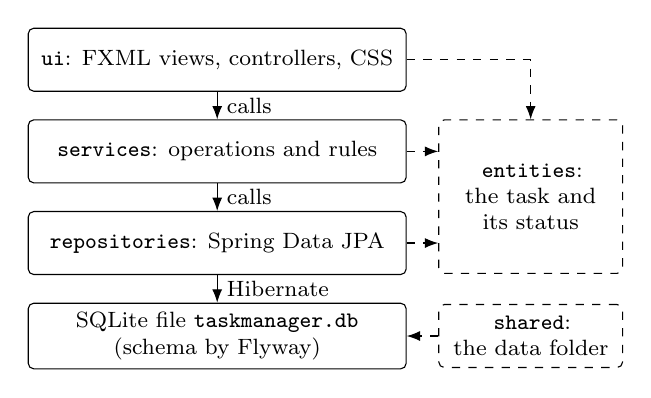
\begin{tikzpicture}[
      node distance=3.5mm and 4mm, >=Latex, font=\footnotesize,
      layer/.style={draw, rounded corners=2pt, minimum width=48mm, minimum height=8mm, align=center},
      side/.style={draw, dashed, rounded corners=2pt, text width=21mm, minimum height=8mm, align=center}]
    \node[layer] (ui) {\texttt{ui}: FXML views, controllers, CSS};
    \node[layer, below=of ui] (services) {\texttt{services}: operations and rules};
    \node[layer, below=of services] (repositories) {\texttt{repositories}: Spring Data JPA};
    \node[layer, below=of repositories] (db) {SQLite file \texttt{taskmanager.db}\\(schema by Flyway)};
    \node[side, right=of services, yshift=-5.75mm, minimum height=19.5mm] (entities)
      {\texttt{entities}:\\the task and its status};
    \node[side, right=of db] (shared) {\texttt{shared}:\\the data folder};
    \draw[->] (ui) -- node[right] {calls} (services);
    \draw[->] (services) -- node[right] {calls} (repositories);
    \draw[->] (repositories) -- node[right] {Hibernate} (db);
    \draw[->, dashed] (services.east) -- (services.east -| entities.west);
    \draw[->, dashed] (repositories.east) -- (repositories.east -| entities.west);
    \draw[->, dashed] (shared) -- (db);
    \draw[->, dashed] (ui.east) -| (entities.north);
  \end{tikzpicture}
  \caption{The layers of the program, in package \texttt{io.mcs.taskmanager}. Screens call services, never
           repositories; a dashed arrow means ``uses''.}\label{fig:layers}
\end{figure}

\subsection{Spring under JavaFX}

The program is a JavaFX application running on top of a Spring Boot application context with no web server. The
main class, \texttt{TaskManagerApplication}, is the Spring Boot application class, but it does not itself extend
JavaFX's \texttt{Application}: when the program is started from a plain class path, as Maven and the IDE start it, a
main class that extends \texttt{Application} stops with an error saying that the JavaFX runtime components are
missing. Its \texttt{main} method therefore hands over to a separate JavaFX application class, \texttt{ui.DesktopApp},
through \texttt{Application.launch}. JavaFX then calls three of its methods in turn:
\begin{itemize}
  \item \texttt{init()} starts Spring, before the window opens, with the data folder from \texttt{AppDataFolder}, so
        that the database has been found or made and migrated by Flyway by then;
  \item \texttt{start(Stage)} loads the window's FXML with Spring as the FXML loader's controller factory, so the
        window's controller is a Spring bean, then applies the stylesheet and shows the window;
  \item \texttt{stop()} closes Spring once the window has closed, and with it the database.
\end{itemize}
Because the controller is a Spring bean, it is handed the task service through its constructor, like any other bean,
and never creates it itself.

\subsection{Persistence}

Tasks are kept in an SQLite database~\cite{sqlite}, a single file that needs no server and no installation:
\path{%LOCALAPPDATA%\TaskManager\taskmanager.db}. The folder belongs to the signed-in Windows user and can be written
without administrator rights, and it is local rather than roaming, so the database is not copied around with the
user's profile.

The schema is created by Flyway~\cite{flyway} from versioned SQL scripts in
\path{src/main/resources/db/migration}, which run every time the program starts and apply any script the database
has not yet seen. Hibernate~\cite{hibernate} maps the task entity onto the table the scripts made, and only checks
that the two match (\texttt{spring.jpa.hibernate.ddl-auto=validate}); it never changes the schema itself. Spring
Data JPA~\cite{spring-boot} generates the repository's implementation from its interface.

Two copies of the program may have the same file open, and the connection is set up for it (Listing~\ref{lst:url}).
The database is opened in SQLite's write-ahead-log mode, which lets one copy read the file while the other writes.
Every transaction begins by taking the write lock (\texttt{transaction\_mode=IMMEDIATE}), so a copy that has read a
task saves its change before the other copy can change or delete that task, and a write that finds the lock taken
waits up to five seconds (\texttt{busy\_timeout=5000}) instead of failing at once. Each copy uses a single
connection, since SQLite takes one writer at a time anyway. This is what makes the two-copy scenario of
Section~\ref{sec:problem} safe to run.

\source[firstline=11, lastline=14, language={}]{src/main/resources/application.properties}
  {The connection, in \texttt{application.properties}}{lst:url}

\subsection{Rules and errors}

Every rule a change must pass is checked in a service: that the title is not blank once trimmed, that the title and
the description are within their length limits, and that the task still exists. A change the program will not make
is refused with one exception type, \texttt{Refused}, an unchecked exception whose message is written for the user,
such as ``A task needs a title, such as "Submit the OEL report".'' The service throws it inside its transaction, so
nothing of the refused change is saved; the screen catches it and shows the message as it is.

Keeping the rules in the services means that each rule lives in exactly one place, that the screens stay free of
rules, and that the JUnit tests exercise the same rules the user meets, without opening a window.

The entity's Bean Validation annotations stay as a last check behind the service, but they are not a way to refuse a
change: Hibernate checks them when it writes the task, which here is when the transaction commits, and a failure
there arrives as a \texttt{TransactionSystemException} with no message meant for the user. This is why the length limits are checked in
the service, with their own messages. Before they were, a title of 101 characters got past the service and failed
only at the commit (Section~\ref{sec:git} shows the change that fixed it).
An error the service does not expect, which is not a \texttt{Refused}, is caught by the screen, written to the log,
and shown as one plain sentence; how the user meets each kind of error is described in
Section~\ref{sec:functionality}.

\subsection{Reasons for the design}

\paragraph*{JavaFX rather than Swing} The brief allows either. JavaFX~\cite{openjfx} keeps the layout of each view in an FXML file
and its look in a CSS stylesheet, apart from the Java code, and its table and list controls are bound to observable
lists that redraw themselves when the data changes.

\paragraph*{Spring rather than objects wired by hand} With Spring, services and controllers are handed their
collaborators instead of constructing them, each service operation runs in a transaction, and the tests start the
same application context, with the same services and rules, on a database of their own.

\paragraph*{SQLite rather than a text file} A database gives transactions, so a change is saved completely or not at
all, and it lets two copies of the program share the data safely. SQLite gives this without a server.

\paragraph*{Flyway rather than letting Hibernate create the tables} The schema is versioned together with the code,
and every database, the user's and each test's, is built by the same scripts. Because Hibernate only validates, a
mismatch between the code and the schema stops the program when it starts instead of surfacing later as a failed
save.

\paragraph*{No code generation for accessors} Every constructor, getter and setter is written out by hand rather than
generated by a library such as Lombok, because the Javadoc tool reads the source: only members that are in the source
can be documented.

\section{Data Structures and Algorithms}\label{sec:dsa}

This section describes how a task is represented, in the database and in memory, and the algorithms behind the
program's operations.

\subsection{The task}

A task is an instance of the JPA entity \texttt{Task} in package \texttt{entities}, mapped onto the table
\texttt{tasks}. Table~\ref{tab:task} lists its fields. The two length limits are public constants of the class,
\texttt{Task.MAX\_TITLE\_CHARACTERS} (100) and \texttt{Task.MAX\_DESCRIPTION\_CHARACTERS} (1000), so that the
service and the entity's column definitions use the same numbers. The fields also carry Bean Validation
annotations (\texttt{@NotBlank}, \texttt{@NotNull}, \texttt{@Size}); they are not where the rules are enforced, which
is the service, but a last check that stops a task that slipped past the service from reaching the database.

\begin{table}[!t]
  \caption{The fields of a task}\label{tab:task}
  \centering\footnotesize
  \begin{tabularx}{\linewidth}{@{}L{0.2\linewidth}L{0.16\linewidth}L{0.25\linewidth}Y@{}}
    \toprule
    Field & Java type & Column & Rule \\
    \midrule
    \texttt{id} & \texttt{UUID} & \texttt{id char(36)}, primary key & Given by Hibernate on the first save; never
      changed, so it has no setter. \\
    \texttt{title} & \texttt{String} & \texttt{title varchar(100)} & Not blank; trimmed; at most 100 characters. \\
    \texttt{description} & \texttt{String} & \texttt{description varchar(1000)} & Trimmed; at most 1000
      characters; empty, never null, when there is none. \\
    \texttt{status} & \texttt{TaskStatus} & \texttt{status varchar(16)} & A new task is Pending. \\
    \texttt{createdAt} & \texttt{Instant} & \texttt{created\_at timestamp} & Set when the task is added; never
      written again. \\
    \texttt{updatedAt} & \texttt{Instant} & \texttt{updated\_at timestamp} & Equal to \texttt{createdAt} at first;
      moved on by every update and status change. \\
    \bottomrule
  \end{tabularx}
\end{table}

Every column is \texttt{not null}. The identifier is a random UUID rather than a counter, stored as 36 characters,
and the two times are \texttt{Instant}s, moments in UTC that the screen shows in the computer's own time zone.

\subsection{The status}

The status is the enum \texttt{TaskStatus} with three constants, \texttt{PENDING}, \texttt{IN\_PROGRESS} and
\texttt{COMPLETED}. Each carries the words the screen shows for it (``Pending'', ``In Progress'', ``Completed''),
returned by \texttt{getLabel()} and by \texttt{toString()}, so a list or a choice box of statuses shows the words
without any conversion. The database keeps the constant's name (\texttt{@Enumerated(EnumType.STRING)}), not its
position, so reordering the constants or changing a label never changes what a saved task means.

\subsection{The table}

The table is created by the first Flyway migration, Listing~\ref{lst:v1}, which is the whole schema of the program.

\source[language=SQL, morekeywords={char,varchar,timestamp}]{src/main/resources/db/migration/V1__tasks.sql}
  {The migration \texttt{V1\_\_tasks.sql}}{lst:v1}

\subsection{The counts}

The number of tasks in each status is returned by the service as a record,
\texttt{TaskCounts(long pending, long inProgress, long completed)}, with two methods of its own: \texttt{total()}, the
number of tasks in all, and \texttt{of(TaskStatus)}, the count for one status, which lets the screen go through
\texttt{TaskStatus.values()} instead of naming each status.

\subsection{Collections in the interface}

The window shows the tasks in a JavaFX \texttt{ListView<Task>}, whose rows are drawn by a cell class of the
program's own, \texttt{TaskCell}. Its items are an observable list, which the list redraws whenever it changes. The
screen keeps no copy of the tasks to filter or count itself: after every change, and whenever the search text or the
filter changes, it asks the service again for the matching tasks and the counts, and replaces the list's items with
the answer, choosing the same task again if it is still listed. What the window shows is therefore always what is
saved, including what a second copy of the program has changed, once the list is read again. Times are shown in the
computer's own time zone, as ``Today, 21:40'', ``Yesterday, 09:05'', ``16 Nov, 14:00'' or, in another year,
``16 Nov 2025, 14:00''.

\subsection{Algorithms}

\paragraph*{Validation} Every save of a title and a description goes through one private method of the service,
\texttt{set}. It trims both texts with \texttt{String.strip()}, which removes spaces, tabs and line breaks around
them, and turns a missing description into an empty one. It then refuses, in this order, an empty title, a title over
100 characters and a description over 1000, each with its own message. The limits are counted after trimming, so
spaces typed around a text never push it over. An update checks before this that a task was chosen and still exists,
and after it that a status was given.

\paragraph*{Listing and ordering} The list is every task, newest first. The repository declares the method
\texttt{findAllByOrderByCreatedAtDesc()}, and Spring Data derives the query from its name.

\paragraph*{Search and filter} Searching and filtering are one database query (Listing~\ref{lst:search}). The service
trims the search text, lowers its case, and wraps it as a \texttt{like} pattern, \texttt{\%text\%}, matched against
the lowered title and the lowered description. The characters \texttt{\%} and \texttt{\_}, which are wildcards in a
\texttt{like} pattern, and \texttt{!}, chosen as the escape character, are escaped first, so that every character the
user types is matched as it is. A blank search becomes \texttt{\%\%}, which matches every task, and a status of
\texttt{null} means every status, so the same query serves the plain list, a search, a filter and both together.
Case is ignored only for the letters A to Z, because SQLite's \texttt{lower()} function folds ASCII letters only.

\source[firstline=28, lastline=42, gobble=4]{src/main/java/io/mcs/taskmanager/repositories/TaskRepository.java}
  {The search query in \texttt{TaskRepository}}{lst:search}

\paragraph*{Counts per status} The service counts each status with the derived query
\texttt{countByStatus(TaskStatus)}, three queries in one read-only transaction. The counts are always over every task,
whatever the search or filter shows.

\paragraph*{A task that no longer exists} Every operation on one task (opening it, updating it, changing its status
and deleting it) first looks it up through one private method, \texttt{find}. A missing identifier is refused with ``Choose a task in
the list first.'', and a task the database no longer has with ``This task no longer exists: it may have been deleted
in another copy of the Task Manager.'' Because each service method is one transaction and the
database begins every transaction by taking its write lock (\texttt{transaction\_mode=IMMEDIATE} in the connection
URL), the other copy of the program cannot delete the task between this lookup and the save that follows it; its
delete waits until the save is done. How this was found and fixed is told in Section~\ref{sec:git}.

\paragraph*{Cost} With $n$ tasks, listing, searching and counting each read the whole table, $O(n)$: a pattern that
starts with \texttt{\%} cannot use an index, and the list is short enough that none is needed. Finding one task by its
identifier uses the index SQLite keeps on the primary key, $O(\log n)$.

\section{Program Functionality}\label{sec:functionality}

This section walks through the program as the user meets it, one function at a time, with a screenshot of each. The
screenshots of the brief's test cases are referred to again in Section~\ref{sec:testing}.

The program has a single window (Fig.~\ref{fig:app-05-all-tasks}). Its header takes the place of the system's title
bar and carries the program's mark and name, with the system's minimise, maximise and close buttons drawn on it. A
sidebar on the left lists the filters under \emph{Tasks}: All tasks, Pending, In Progress and Completed, each with the
number of tasks it holds, so that the counts per status are always in view. At the sidebar's foot is the list of
keyboard shortcuts. The rest of the window is the list: a heading (``All tasks'', or the status the list is filtered
by) with a line under it saying what the list shows, such as ``4 tasks, newest first.'', the \emph{Refresh} and
\emph{Add task} buttons, the search field (``Search titles and descriptions''), and the tasks, one row each, under the
columns Task, Status and Updated. The row under the pointer, and the chosen row, show an \emph{Edit} and a
\emph{Delete} button at their end. Forms and confirmations open as dialogs over the window, which is dimmed behind
them. A notice the program has to give, such as a task that no longer exists, appears as a red bar over the list,
with a \emph{Dismiss} button.

\subsection{An empty list}

When there are no tasks, the list is replaced by a message: ``No tasks yet'', with the hint ``Add your first with Add
task or Ctrl+N, such as “Submit the OEL report”.'' (Fig.~\ref{fig:app-01-empty-list}). A search or a filter that
matches nothing says so in the same place: ``Nothing matches “report”'' for a search, or ``No pending tasks'' and the
like for an empty status.

\screenshotwide{app-01-empty-list}
  {The window with no tasks: the list shows a message instead of an empty table (test case 4).}
  {Test case 4: the empty list and its message}

\subsection{Adding a task}

The \emph{Add task} button, or Ctrl+N, opens the form for a new task (Fig.~\ref{fig:app-02-add-form}). It has a
\emph{Title} and a \emph{Description} field, each with a count of its characters against its limit, ``12 / 100'' for
example, counted after trimming as the service counts them and turning red past the limit, and the note ``It starts
as Pending; change its status from the list as the work goes.'' The \emph{Add task} button in the form saves it (as do
Enter in the title and Ctrl+Enter anywhere in the form), and \emph{Cancel} or Esc closes the form without saving. The new task appears at
the top of the list, chosen (Fig.~\ref{fig:app-03-task-added}).

\screenshot{app-02-add-form}
  {The form for a new task, filled in for a second task.}
  {The add form filled in}

\screenshotwide{app-03-task-added}
  {The first task, ``Task 1'', added to the list (test case 1).}
  {Test case 1: the new task in the list}

A title left empty, or made only of spaces, is refused by the service, and its message is shown in the form under the
fields: ``A task needs a title, such as "Submit the OEL report".'' (Fig.~\ref{fig:app-04-empty-title}). The form stays
open with what was typed, so the user can correct it. A title over 100 characters or a description over 1000 is
refused the same way, with a message giving the limit and the length typed.

\screenshot{app-04-empty-title}
  {Saving a task with a description but no title: the form shows ``A task needs a title, such as "Submit the OEL
   report".'' (test case 2).}
  {Test case 2: the validation message}

\subsection{Viewing all tasks}

All tasks are listed newest first (Fig.~\ref{fig:app-05-all-tasks}). Each row shows the title, the first line of the
description, the status, when the task was last updated and when it was added, the times written as ``Today, 21:40'',
``Yesterday, 09:05'' or a date. The status is a coloured pill, grey for Pending, blue for In Progress and green
for Completed, and a completed task's title is greyed and struck through.

\screenshotwide{app-05-all-tasks}
  {Three tasks, one in each status; the sidebar counts 1, 1 and 1 (test case 3).}
  {Test case 3: several tasks, all three statuses}

\subsection{Updating a task}

The row's \emph{Edit} button, Enter on the chosen row, a double click or the row's right-click menu opens the edit
form on the task as it is saved now (Fig.~\ref{fig:app-06-edit-form}). It has the same two fields and a \emph{Status}
choice of Pending, In Progress and Completed, and notes when the task was added and last changed. \emph{Save} saves
all three at once
(Fig.~\ref{fig:app-07-task-updated}).

\screenshot{app-06-edit-form}
  {The edit form on an existing task.}
  {The edit form on an existing task}

\screenshotwide{app-07-task-updated}
  {The task with its changed details in the list (test case 5).}
  {Test case 5: the changed details in the list}

If the task has been deleted in a second copy of the program while the form was open, saving closes the form, shows
the service's message over the list, ``This task no longer exists: it may have been deleted in another copy of the
Task Manager.'', and reads the list again, which no longer has the task (Fig.~\ref{fig:app-08-update-missing}). The
same happens when such a task is opened for editing, deleted or given a new status.

\screenshotwide{app-08-update-missing}
  {Saving a change to a task that a second copy of the program has deleted: the red notice says the task no longer
   exists, and the list, read again, shows the two tasks that remain (test cases 6 and 7).}
  {Test case 6: the message for a task that no longer exists}

\subsection{Deleting a task}

The row's \emph{Delete} button, the Delete key on the chosen row, or \emph{Delete task} in the edit form asks first:
a dialog titled ``Delete this task?'' says ``“Submit the OEL report” will be deleted for good. This can't be
undone.'', naming the task, with \emph{Cancel} and \emph{Delete task} buttons (Fig.~\ref{fig:app-09-delete-confirm}). Only \emph{Delete task} deletes it, and the task then disappears from the list, as Fig.~\ref{fig:app-08-update-missing}
shows for the task deleted in the second copy.

\screenshot{app-09-delete-confirm}
  {The confirmation before ``Task 4'' is deleted.}
  {The delete confirmation}

\subsection{Changing the status from the list}

The status in each row is a button: it opens a menu of the three statuses with the task's own ticked, and choosing
another moves the task to it at once, without opening the form. The counts in the sidebar follow, and the filter for
the new status lists the task (Fig.~\ref{fig:app-11-status-change}).

\screenshotwide{app-11-status-change}
  {The In Progress filter chosen in the sidebar, listing the task whose status was changed from the list; the counts
   are 1, 1 and 1.}
  {A status changed from the list, counts updated}

\subsection{Searching and filtering}

Typing in the search field narrows the list, as each character is typed, to the tasks whose title or description
holds the text, whatever its case (Fig.~\ref{fig:app-12-search-filter}); Ctrl+F goes to the field, Esc clears it, and
the down arrow moves into the list. Choosing a filter in the sidebar shows
one status only, and the two combine: the line under the heading then says, for example, ``2 of 5 pending tasks
match “report”.''

\screenshotwide{app-12-search-filter}
  {A search for ``3'' narrowing the list to one of the three tasks.}
  {Search and status filter narrowing the list}

\subsection{Keyboard shortcuts}

Table~\ref{tab:shortcuts} lists the keyboard shortcuts. The sidebar shows the five that work in the window: add,
edit, delete, search and refresh.

\begin{table}[!t]
  \caption{Keyboard shortcuts}\label{tab:shortcuts}
  \centering\footnotesize
  \begin{tabularx}{\linewidth}{@{}YL{0.2\linewidth}L{0.36\linewidth}@{}}
    \toprule
    Action & Key & Where \\
    \midrule
    Add a task & Ctrl+N & Anywhere in the window \\
    Edit the chosen task & Enter & In the list \\
    Delete the chosen task & Delete & In the list \\
    Go to the search & Ctrl+F & Anywhere in the window \\
    Clear the search & Esc & In the search field \\
    Read the list again & F5 & Anywhere in the window \\
    Save the form & Ctrl+Enter & Anywhere in a form \\
    Save the form & Enter & In the title field \\
    Close a form without saving & Esc & In a form \\
    \bottomrule
  \end{tabularx}
\end{table}

\subsection{Error handling}

The user meets three kinds of error, and none of them as a stack trace. A change the service refuses shows the
service's own message: in the form, under its fields, for a form, or over the list for a change made from the list. A
task that no longer exists is reported over the list, which is then read again. Any other failure, which nobody
expects, such as the database not answering, is written to the log and shown over the list as one plain sentence:
``Something went wrong, and nothing was changed. Try again, or restart the Task Manager if it keeps happening.'' The
same holds for an exception nobody caught on the window's thread, which the program hands to the window instead of
letting it print.

\section{Development in the IDE}\label{sec:ide}

\subsection{Setting up the project}

The project was created as a Maven project with the Maven wrapper and opened in Visual Studio Code as a folder. The
Java extension reads \texttt{pom.xml}, imports the project with its dependencies, and compiles it in the background;
errors and warnings appear in the editor as the code is typed. Fig.~\ref{fig:ide-01-project} shows the project open,
its folders in the Explorer and the integrated terminal below the editor.

\screenshotwide{ide-01-project}
  {The project open in Visual Studio Code: the project tree in the Explorer, and the integrated terminal after a run of
   the Javadoc tool.}
  {VS Code with the project open: Explorer tree, Java Projects view, JDK 25}

The folder holds the Maven wrapper (\texttt{mvnw}, \texttt{mvnw.cmd} and \path{.mvn/}), \texttt{pom.xml}, the
IDE's settings in \path{.vscode/}, and the README. The code is under \path{src/main/java}, its resources (the
settings, the Flyway migration, and the window's FXML, stylesheet and fonts) under \path{src/main/resources}, and the
tests under \path{src/test/java}. The generated documentation is in \path{docs/javadoc/}, and this report in
\path{report/}.

\subsection{Running the program}

The project carries a launch configuration for the IDE, ``Task Manager'' in \path{.vscode/launch.json}: it starts
the main class \texttt{io.mcs.taskmanager.TaskManagerApplication} on JDK~25 with
\texttt{--enable-native-access=ALL-UNNAMED}, from the Run and Debug view or with F5, and shows the program's output in
the Debug Console. The program also starts from the IDE's integrated terminal with the Maven wrapper,
\texttt{.\textbackslash{}mvnw.cmd spring-boot:run} in PowerShell or \texttt{./mvnw spring-boot:run} in Git Bash.
Fig.~\ref{fig:ide-02-run} shows it started that way: its window, on the empty list, open over the editor, and
Spring's start-up line in the terminal behind it.

\screenshotwide{ide-02-run}
  {The program started from the IDE's integrated terminal with \texttt{.\textbackslash{}mvnw.cmd spring-boot:run}: its window, on
   the empty list, over the editor.}
  {The app started from the terminal}

\subsection{Debugging}

Because the launch configuration is of type \texttt{java}, the IDE starts the program under the Java debugger: a
breakpoint set in the editor, for example on the first line of \texttt{TaskService.create}, stops the program there
when a task is added, and the Variables and Call Stack views then show its state, from which it can be stepped
through line by line.

\section{Version Control with Git}\label{sec:git}

The project's history is kept in a Git repository~\cite{progit} and published on GitHub at
\RepoURL, branch \texttt{main}. All commands were run in a terminal in the project folder.

\subsection{Setting up the repository}

The repository was created as soon as the project skeleton existed: the Maven wrapper, \texttt{pom.xml}, the
application class and the IDE's launch configuration. The steps were:
\begin{enumerate}
  \item \texttt{git init -b main}: create an empty repository whose first branch is \texttt{main};
  \item \texttt{git status}: check which files Git sees, all of them untracked at this point;
  \item \texttt{git add .}: stage the whole skeleton for the first commit, the build output and the local database
        being kept out by \texttt{.gitignore};
  \item \texttt{git status}: check that exactly the intended files are staged;
  \item \texttt{git commit}: record the initial commit;
  \item \texttt{git remote add origin} with the GitHub address, then \texttt{git remote -v} to check it;
  \item \texttt{git push -u origin main}: publish the branch and make \texttt{origin/main} its upstream.
\end{enumerate}
Listing~\ref{lst:01-initial-setup.txt} is the transcript of the first four steps as they ran.

\evidence[firstline=1, lastline=52]{01-initial-setup.txt}
  {Creating the repository and staging the skeleton}

The warnings printed by \texttt{git add} are Git for Windows noting that the files, written with Unix line endings,
will be checked out with Windows ones; they do not affect what is committed.

The last three steps are seen best in the repository as it is now (Listing~\ref{lst:remote}): the first commit
of the history is still the initial one, \texttt{origin} points at the GitHub repository, and \texttt{main} tracks
\texttt{origin/main}, with nothing committed that has not been pushed. (The untracked \texttt{report/} folder is
this report, before its own commit.)

\begin{lstlisting}[style=terminal, caption={The initial commit, the remote and the tracking branch, in the live
repository}, label={lst:remote}]
$ git log --reverse --format="%h %ad %s" --date=short | head -n 1
a0bb38c 2026-11-22 Initial commit: Spring Boot and JavaFX project skeleton on Maven

$ git remote -v
origin	https://github.com/hamdotexe/taskmanager.git (fetch)
origin	https://github.com/hamdotexe/taskmanager.git (push)

$ git status -sb
## main...origin/main
?? report/
\end{lstlisting}

\subsection{The workflow for each change}

Each piece of work, such as a new rule in the service, a screen, or a fix, was committed on its own, in this order:
\begin{enumerate}
  \item \texttt{git status}: see which files the change touched;
  \item \texttt{git diff}: read every changed line before staging it;
  \item \texttt{./mvnw -q test}: run the tests; nothing is committed unless they pass;
  \item \texttt{git add} followed by the files of the change, named one by one: staging by explicit path keeps
        unrelated edits and generated files out of the commit;
  \item \texttt{git commit -m "Area: what changed and why"}, with a second \texttt{-m} for a body when the reason
        needs more than a line;
  \item \texttt{git push}: publish the commit to \texttt{origin/main}.
\end{enumerate}
The history as a whole is reviewed with \texttt{git log --oneline --graph}, one line per commit.

\subsection{Commit messages}

Every message starts with the area of the program it changes, followed by what changed and, where it is not obvious,
why: for example ``Tasks: change a task's status on its own, as the list will'' or ``Test: tasks survive a restart of
the app''. A message that names its area makes the one-line log readable as a list of the program's parts as they
were built. When the reason needs more than a line, a body after a blank line gives it, as in this commit from the
history:
\begin{lstlisting}[style=terminal]
Tasks: trim the title and description, and refuse either over its limit

A title over 100 characters or a description over 1000 got past the service
and failed Bean Validation at commit, so the screen would have had a
TransactionSystemException to show. The service now refuses them with the
limit and the length typed, counted after trimming, so spaces around a text
never push it over. No description is kept as empty.

TaskRulesTest covers blank and missing titles, trimming, both limits at and
past the edge, a refused update leaving the task as it was, and a change
with no task chosen.
\end{lstlisting}

\subsection{Recording revisions: status, diff and log}

Three times during development, for a new rule and for two bug fixes, the output of \texttt{git status} and
\texttt{git diff} was saved with its commands just before the change was staged. In each, \texttt{git status} also
lists the \texttt{report/} folder as untracked: this report was being written at the same time and was committed on
its own.

\paragraph*{A new rule} A title over 100 characters or a description over 1000 used to get past the service and fail
Bean Validation at the commit, as described in Section~\ref{sec:design}. Listing~\ref{lst:02-status-diff-title-limits.txt}
shows the change that moved both limits into the service: \texttt{git status} lists the modified
\texttt{TaskService.java} and the new, still untracked test class \texttt{TaskRulesTest.java}, and \texttt{git diff}
shows the method \texttt{set} now trimming both texts and refusing either one over its limit, with the length typed in
the message.

\evidence[linerange={1-22,68-112}]{02-status-diff-title-limits.txt}
  {\texttt{git status} and \texttt{git diff} before the length limits were committed (the hunks that change only
   comments, lines 23--67 of the transcript, are left out)}

\paragraph*{A bug fix} With two copies of the program open on one file, a copy that had read a task could not save it
once the other copy had written in between: SQLite refused the write at once with \texttt{SQLITE\_BUSY\_SNAPSHOT},
the busy timeout did not help, and the save failed with a raw \texttt{CannotAcquireLockException} rather than a
message.
A new test, \texttt{TwoCopiesTest}, reproduced it with a second Spring context on the same database playing the other
copy. The fix is one setting in the connection URL (Listing~\ref{lst:03-status-diff-two-copies-fix.txt}): every
transaction now takes the write lock as it begins, so the other copy's change waits for this one to finish and then
goes through.

\evidence{03-status-diff-two-copies-fix.txt}
  {\texttt{git status} and \texttt{git diff} before the fix for two copies was committed}

\paragraph*{A bug fix in the window} When a dialog opened, the keyboard did not go to its first field: Ctrl+N
followed by typing lost the first keys, and the focus stayed in the list. The dimmed layer the dialog sits on is a
scroll pane, which puts its content in the window only once its skin is made, on the next pass of the stylesheet, so
asking the title field for the focus before then did nothing. The fix applies the stylesheet first
(Listing~\ref{lst:04-status-diff-dialog-focus-fix.txt}). This time \texttt{git diff} was given the one file of the
fix; \texttt{git status} shows the other files then changed, which went into commits of their own.

\evidence{04-status-diff-dialog-focus-fix.txt}
  {\texttt{git status} and \texttt{git diff} before the fix for the dialog's focus was committed}

Figures~\ref{fig:git-02-add-commit-push} to~\ref{fig:git-04-github} show the workflow in the terminal and on GitHub.
In Fig.~\ref{fig:git-02-add-commit-push}, a change to the README (the group's members) and to \texttt{pom.xml} (the
Spring Boot patch version, 4.1.2 to 4.1.3) is checked with \texttt{git status}, staged with \texttt{git add .}, which
with only those two files changed stages exactly them, committed and pushed. Fig.~\ref{fig:git-03-log} shows the
whole history as a graph, and Fig.~\ref{fig:git-04-github} the commits as GitHub lists them. The diffs themselves are
in the listings above.

\screenshotwide{git-02-add-commit-push}
  {A change checked with \texttt{git status} (README.md and pom.xml modified), then staged, committed and pushed
   with \texttt{git add}, \texttt{git commit} and \texttt{git push} (c1479d6..ae85057).}
  {Terminal: git add, git commit, git push of that change}

\screenshotwide{git-03-log}
  {The whole history with \texttt{git log --oneline --graph}: 22 commits, \texttt{HEAD} at ae85057.}
  {Terminal: \texttt{git log --oneline --graph} of the whole history}

\screenshotwide{git-04-github}
  {The repository's commits on GitHub.}
  {The repository's commits page on GitHub}

\subsection{The history}

When this report was built, the history had \CommitCount\ commits, made between \FirstCommitDate\ and
\LastCommitDate.
Table~\ref{tab:history} lists them oldest first, with the first line of each message, as
\texttt{git log --reverse} prints them.

\begin{table*}[!tp]
  \caption{The commit history}\label{tab:history}
  \centering\footnotesize
  \begin{tabularx}{\textwidth}{@{}rlL{0.15\textwidth}Y@{}}
    \toprule
    No. & Commit & Date & Message (first line) \\
    \midrule
    \CommitRows
    \bottomrule
  \end{tabularx}
\end{table*}

\section{Documentation with Javadoc}\label{sec:javadoc}

\subsection{Comments in the code}

Every class, interface, enum and record, every constructor and every method carries a Javadoc comment, private
members and the handlers the FXML views call included. The comments follow the conventions of the documentation
comment specification~\cite{doc-comment-spec}:
\begin{itemize}
  \item the first sentence says what the element is or does, and becomes its summary in the generated pages;
  \item each parameter is described with \texttt{@param}, and the result of every method that returns one with
        \texttt{@return};
  \item an exception the method throws on purpose is described with \texttt{@throws}, saying when;
  \item every type names its two authors, one \texttt{@author} tag each: \texttt{@author Hamza Rasool} and
        \texttt{@author Abdullah Khan}.
\end{itemize}
Listing~\ref{lst:javadoc} shows the class comment of the task service and the comment of its \texttt{create} method,
as they are in the source.

\source[linerange={15-29,91-108}, gobble=0]{src/main/java/io/mcs/taskmanager/services/TaskService.java}
  {Javadoc comments in \texttt{TaskService}: the class and its \texttt{create} method}{lst:javadoc}
% Check after any change to TaskService: lines 15-29 are the class comment and 91-108 create.

\subsection{Generating the HTML}

The HTML documentation is generated by the Javadoc tool~\cite{javadoc-tool} through the Maven Javadoc Plugin, with one
command from the project folder:
\begin{center}
  \texttt{./mvnw javadoc:javadoc}
\end{center}
The plugin's configuration in \texttt{pom.xml} (Listing~\ref{lst:javadoc-plugin}) turns on every check doclint has
and makes any warning fail the build rather than scroll past, includes private members, shows the \texttt{@author}
tags, and leaves the date out of the pages, so that generating them again changes only what the code changed. The
pages are written into the repository, under \path{docs/javadoc/apidocs/}, and committed with the code, so they are
part of the submission.

\source[firstline=106, lastline=126, gobble=3, tabsize=4, language=XML]{pom.xml}
  {The Maven Javadoc Plugin's configuration in \texttt{pom.xml}}{lst:javadoc-plugin}

Because a single warning would fail it, a run that ends in BUILD SUCCESS means that every comment passed every check.
The last run before this report was built printed no warning at all:
\begin{lstlisting}[style=terminal, literate={-}{{-\allowbreak}}1]
$ ./mvnw javadoc:javadoc
...
[INFO] --- javadoc:3.12.0:javadoc (default-cli) @ taskmanager ---
[INFO] ------------------------------------------------------------------------
[INFO] BUILD SUCCESS
[INFO] ------------------------------------------------------------------------
[INFO] Total time:  3.302 s
[INFO] Finished at: 2026-11-22T22:50:32+05:00
\end{lstlisting}

\screenshotwide{javadoc-01-generate}
  {Generating the documentation with \texttt{./mvnw javadoc:javadoc}, ending in BUILD SUCCESS.}
  {Terminal: ./mvnw javadoc:javadoc ending in BUILD SUCCESS}

\subsection{Reviewing it in a browser}

The generated pages were opened from \path{docs/javadoc/apidocs/index.html} in a web browser and reviewed there. The
overview lists the seven packages, \texttt{io.mcs.taskmanager} and its \texttt{entities}, \texttt{repositories},
\texttt{services}, \texttt{shared}, \texttt{ui} and \texttt{ui.kit}, each with the summary from its
\texttt{package-info.java} (Fig.~\ref{fig:javadoc-02-index}). Each class page lists its fields, constructors and
methods, private ones included, with their parameters, return values and exceptions, and names the class's authors
(Fig.~\ref{fig:javadoc-03-class}). The documentation is 71 HTML pages in all, with an index and a search.
% VERIFY in phase 3: the screenshots show this.

\screenshotwide{javadoc-02-index}
  {The generated documentation's overview page, \texttt{docs/javadoc/apidocs/index.html}, in a browser.}
  {docs/javadoc/apidocs/index.html in a browser}

\screenshotwide{javadoc-03-class}
  {The task service's page: method details with their parameters and return values.}
  {The task service's page in the browser, method details with parameters and returns}

\section{Testing}\label{sec:testing}

\subsection{Approach}

The program was tested at two levels.

\paragraph*{Automated tests} JUnit tests~\cite{junit}, run through Spring Boot's test support, start the
application's Spring context without opening a window and call the task service exactly as the screens do, so they
exercise the same rules the user meets. Most test classes extend \texttt{DatabaseTestBase}, which gives each class a
new, empty database in a temporary folder: Flyway runs the migration on it and Hibernate checks the entity against
the table, as when the program starts for the first time. The context is closed after each class, so that its
connection lets go of the file before JUnit deletes the folder, which Windows would otherwise refuse. Two classes
start further contexts of their own: \texttt{RestartTest} starts the program's Spring side on a folder, adds a task,
closes it and starts it again on the same folder, and \texttt{TwoCopiesTest} opens a second context on the same
database to play the second copy of the program in test case 6.

A seventh class, \texttt{TaskTextTest}, needs neither Spring nor a window: it checks the words the screen puts
together, such as how a time is written and what an empty list says, by calling \texttt{TaskText} directly. The tests
are organised in these seven classes:
\begin{itemize}
  \item \texttt{BriefTestCasesTest}: the brief's seven test cases, one test each, in the brief's order;
  \item \texttt{TaskRulesTest}: the rules a task is saved under, beyond the brief's cases;
  \item \texttt{SearchAndCountsTest}: the search, the status filter and the counts;
  \item \texttt{TwoCopiesTest}: two copies of the program on one database;
  \item \texttt{RestartTest}: tasks surviving a restart;
  \item \texttt{FoundationTest}: the program starting on an empty database;
  \item \texttt{TaskTextTest}: the words the window shows.
\end{itemize}
They run with \texttt{./mvnw test}, and \texttt{./mvnw -q test} was run before every commit.

\paragraph*{Tests in the running program} Every test case of the brief was also carried out by hand in the running
program, and the screenshots of Section~\ref{sec:functionality} record what it showed. Test case 6 needs two copies of
the program open on the same database, as explained in Section~\ref{sec:problem}: the first copy opens a task for
editing, the second deletes it, and the first then saves its change.
% VERIFY in phase 3: every manual result in the tables is backed by a screenshot or was observed.

\subsection{The brief's test cases}

Table~\ref{tab:brief-tests} lists the seven test cases of the brief with their expected and actual results, the
steps by which each was carried out in the program, and the JUnit test that checks the same case at the service.

\begin{table*}[!tp]
  \caption{The brief's test cases}\label{tab:brief-tests}
  \centering\footnotesize
  \begin{tabularx}{\textwidth}{@{}L{0.025\textwidth}L{0.12\textwidth}YL{0.17\textwidth}L{0.2\textwidth}L{0.15\textwidth}@{}}
    \toprule
    No. & Test case & Steps in the program & Expected result & JUnit test & Actual result \\
    \midrule
    1 & Add a valid task
      & Click \emph{Add task} (or Ctrl+N), type a title and a description, and click \emph{Add task}.
      & The task is added and appears in the list, Pending.
      & \texttt{tc1AValidTaskIsAdded}
      & JUnit: passed. In the program: \gap{from Fig.~\ref{fig:app-03-task-added}} \\
    2 & Add a task with an empty title
      & Click \emph{Add task}, leave the title empty (or type only spaces), and click \emph{Add task}.
      & A validation message is shown, and no task is added.
      & \texttt{tc2ATaskWithAnEmptyTitle\-IsRefusedWithAMessage}
      & JUnit: passed. In the program: \gap{from Fig.~\ref{fig:app-04-empty-title}} \\
    3 & View all tasks
      & Add several tasks and give them all three statuses from their status menus.
      & All tasks are displayed, each with its status.
      & \texttt{tc3AllTasksAreListed}
      & JUnit: passed. In the program: \gap{from Fig.~\ref{fig:app-05-all-tasks}} \\
    4 & View an empty list
      & Start the program on a database with no tasks.
      & An appropriate message is shown in place of the list.
      & \texttt{tc4AnEmptyListIsEmpty}
      & JUnit: passed. In the program: \gap{from Fig.~\ref{fig:app-01-empty-list}} \\
    5 & Update an existing task
      & Click a task's \emph{Edit}, change its title, description and status, and click \emph{Save}.
      & The task's details are updated in the list.
      & \texttt{tc5AnExistingTaskIsUpdated}
      & JUnit: passed. In the program: \gap{from Fig.~\ref{fig:app-07-task-updated}} \\
    6 & Update a non-existing task
      & With two copies of the program open, click a task's \emph{Edit} in the first, delete the task in the second,
        then click \emph{Save} in the first.
      & Handled gracefully: a message says the task no longer exists, the list is refreshed, and no stack trace is
        shown.
      & \texttt{tc6UpdatingANonExisting\-TaskIsRefusedGracefully}
      & JUnit: passed. In the program: \gap{from Fig.~\ref{fig:app-08-update-missing}} \\
    7 & Delete an existing task
      & Click a task's \emph{Delete}, then \emph{Delete task} in the confirmation.
      & The task is removed from the list.
      & \texttt{tc7AnExistingTaskIsDeleted}
      & JUnit: passed. In the program: \gap{from Fig.~\ref{fig:app-10-task-deleted}} \\
    \bottomrule
  \end{tabularx}
\end{table*}

\subsection{Further test cases}

Table~\ref{tab:more-tests} lists the test cases we added for the requirements of Section~\ref{sec:problem} beyond the
brief's six, one row per JUnit test.

\begin{table*}[!tp]
  \caption{Further test cases}\label{tab:more-tests}
  \centering\footnotesize
  \begin{tabularx}{\textwidth}{@{}L{0.025\textwidth}YL{0.28\textwidth}L{0.27\textwidth}L{0.1\textwidth}@{}}
    \toprule
    No. & Test case & Expected result & JUnit test & Actual result \\
    \midrule
    \multicolumn{5}{@{}l}{\textit{The rules a task is saved under} (\texttt{TaskRulesTest})} \\
    8 & A title of spaces and tabs, or no title at all
      & Refused as an empty title; nothing saved.
      & \texttt{aBlankOrMissingTitleIsRefused} & Passed \\
    9 & Spaces and line breaks around the title and the description
      & Saved without them.
      & \texttt{theTitleAndDescriptionAreTrimmed} & Passed \\
    10 & No description
      & Kept as empty, never as null.
      & \texttt{noDescriptionIsKeptAsEmpty} & Passed \\
    11 & A title of 100 characters, then of 101
      & 100 accepted; 101 refused with a message giving the limit and the length.
      & \texttt{aTitleIsKeptWithinItsLimit} & Passed \\
    12 & A description of 1000 characters, then of 1001
      & 1000 accepted; 1001 refused with a message giving the limit and the length.
      & \texttt{aDescriptionIsKeptWithinItsLimit} & Passed \\
    13 & An update that breaks a rule
      & Refused, and the task is left as it was.
      & \texttt{aRefusedUpdateChangesNothing} & Passed \\
    14 & A status changed from the list, forward and back
      & The status changes; the title and description do not.
      & \texttt{aStatusIsChangedOnItsOwn} & Passed \\
    15 & A status change with no status
      & Refused with a message.
      & \texttt{aStatusChangeWithNoStatus\-IsRefused} & Passed \\
    16 & Changing the status of, deleting, or opening a task that no longer exists
      & Each refused with the message that the task no longer exists.
      & \texttt{aMissingTaskIsRefused\-ByEveryChange} & Passed \\
    17 & A change with no task chosen
      & Refused with ``Choose a task in the list first.''
      & \texttt{noTaskChosenIsRefused} & Passed \\
    \multicolumn{5}{@{}l}{\textit{Search, filter and counts} (\texttt{SearchAndCountsTest})} \\
    18 & Text that is in a title or a description, typed in another case
      & Every task holding it is found.
      & \texttt{searchFindsTheTextInATitle\-OrDescriptionInAnyCase} & Passed \\
    19 & No search text, or only spaces
      & Every task is listed.
      & \texttt{noTextMatchesEveryTask} & Passed \\
    20 & Text that is in no task
      & Nothing is found, and nothing fails.
      & \texttt{textInNoTaskFindsNothing} & Passed \\
    21 & Search text holding \texttt{\%} or \texttt{\_}
      & Matched as typed, not as wildcards.
      & \texttt{wildcardsAreMatchedAsTyped} & Passed \\
    22 & A status chosen in the filter
      & Only the tasks with that status are listed.
      & \texttt{aStatusFilterListsOnlyThatStatus} & Passed \\
    23 & Search text and a status together
      & Only the tasks matching both are listed.
      & \texttt{textAndAStatusNarrowThe\-ListTogether} & Passed \\
    24 & Tasks added, moved between statuses and deleted
      & Each count equals the number of tasks in its status after every change.
      & \texttt{theCountsFollowEveryChange} & Passed \\
    25 & No tasks
      & Every count is 0.
      & \texttt{anEmptyListCountsNothing} & Passed \\
    \multicolumn{5}{@{}l}{\textit{Two copies of the program} (\texttt{TwoCopiesTest})} \\
    26 & The other copy deletes a task; this copy then updates it, changes its status and deletes it
      & Each refused with the message that the task no longer exists; no error.
      & \texttt{aTaskDeletedInTheOtherCopy\-IsRefusedHereWithAMessage} & Passed \\
    27 & One copy adds and changes tasks
      & The other copy reads the changes at once.
      & \texttt{eachCopySeesTheOthersChanges} & Passed \\
    28 & The other copy deletes a task while this copy is saving a change to it
      & The delete waits for the save, then goes through; neither copy fails.
      & \texttt{aDeleteInTheOtherCopy\-WaitsWhileThisCopyIsSaving} & Passed \\
    \multicolumn{5}{@{}l}{\textit{Starting and restarting} (\texttt{RestartTest}, \texttt{FoundationTest})} \\
    29 & A task added and moved on, then the program closed and started again
      & The task is there as it was left.
      & \texttt{tasksSurviveARestart} & Passed \\
    30 & The program started on an empty database
      & Spring starts, Flyway makes the table, and Hibernate finds it as the entity expects.
      & \texttt{startsOnAFreshDatabase} & Passed \\
    \multicolumn{5}{@{}l}{\textit{The words the window shows, without a window} (\texttt{TaskTextTest})} \\
    31 & A time today, yesterday, earlier this year and in another year
      & Written as ``Today, 21:40'', ``Yesterday, 09:05'', ``16 Nov, 14:00'' and ``16 Nov 2025, 14:00''.
      & \texttt{aTimeIsWrittenTheWayThe\-ListWritesIt} & Passed \\
    32 & A moment just after midnight in Karachi, still the day before in UTC
      & Counted on the user's day, not on UTC's.
      & \texttt{theDayIsTheUsersNotUtcs} & Passed \\
    33 & A time inside a sentence
      & ``Today'' and ``Yesterday'' start in lower case; a date stays as it is.
      & \texttt{aTimeInsideASentence\-StartsInLowerCase} & Passed \\
    34 & The list's heading
      & ``All tasks'', or the status filtered by.
      & \texttt{theHeadingNamesWhatIsShown} & Passed \\
    35 & A number of tasks
      & Said with its status, and in the singular for one.
      & \texttt{aNumberOfTasksIsSaid\-WithItsStatus} & Passed \\
    36 & The line under the heading
      & Counts what the filter holds and, with a search, how many of those match.
      & \texttt{theSummarySaysWhat\-TheListShows} & Passed \\
    37 & An empty list
      & Says why: no tasks at all (test case 4), nothing matching the search, or nothing in the status.
      & \texttt{anEmptyListSaysWhy} & Passed \\
    38 & The character count in the form
      & Counted after trimming, as the service counts.
      & \texttt{charactersAreCounted\-AfterTrimming} & Passed \\
    \bottomrule
  \end{tabularx}
\end{table*}

\subsection{Results}

The last run of \texttt{./mvnw test} before this report was built ran all 38 tests, and every one passed:
\begin{lstlisting}[style=terminal]
[INFO] Tests run: 1, Failures: 0, Errors: 0, Skipped: 0, Time elapsed: 7.110 s -- in io.mcs.taskmanager.FoundationTest
[INFO] Tests run: 1, Failures: 0, Errors: 0, Skipped: 0, Time elapsed: 1.435 s -- in io.mcs.taskmanager.RestartTest
[INFO] Tests run: 7, Failures: 0, Errors: 0, Skipped: 0, Time elapsed: 0.798 s -- in io.mcs.taskmanager.services.BriefTestCasesTest
[INFO] Tests run: 8, Failures: 0, Errors: 0, Skipped: 0, Time elapsed: 0.752 s -- in io.mcs.taskmanager.services.SearchAndCountsTest
[INFO] Tests run: 10, Failures: 0, Errors: 0, Skipped: 0, Time elapsed: 0.528 s -- in io.mcs.taskmanager.services.TaskRulesTest
[INFO] Tests run: 3, Failures: 0, Errors: 0, Skipped: 0, Time elapsed: 2.234 s -- in io.mcs.taskmanager.TwoCopiesTest
[INFO] Tests run: 8, Failures: 0, Errors: 0, Skipped: 0, Time elapsed: 0.037 s -- in io.mcs.taskmanager.ui.TaskTextTest
[INFO]
[INFO] Results:
[INFO]
[INFO] Tests run: 38, Failures: 0, Errors: 0, Skipped: 0
[INFO]
[INFO] BUILD SUCCESS
[INFO] Total time:  16.443 s
\end{lstlisting}
These are the lines of that run that report the tests; Spring's log between them is left out. The whole run, Maven's
own start and the compilation included, took 16.4 seconds.

\screenshotwide{test-01-junit}
  {Running the tests with \texttt{./mvnw test}: the totals and BUILD SUCCESS.}
  {Terminal: ./mvnw test with the totals and BUILD SUCCESS}

Two faults were found and fixed while the program was being built, each together with the tests that now cover it:
the length limits that only Bean Validation enforced (test cases 11 and 12), and the save overtaken by a delete in
the other copy (test case 28), which that test reproduced before the fix. Both changes are shown in
Section~\ref{sec:git}.

% every screenshot and table is placed before the conclusion, never after the references
\clearpage
\section{Conclusion}\label{sec:conclusion}

We built Task Manager, a JavaFX desktop application over Spring Boot services that adds, lists, updates and deletes
tasks, sets their status, refuses a task without a title, and keeps its tasks in a local SQLite file. The rules live
in one place, the services, where the JUnit tests check them on a fresh database, and the window only shows what the
services return or refuse. All 38 tests pass, the Javadoc HTML is generated with every check on and not one warning,
and the history records the work as \CommitCount\ commits, each with a message that says what changed and why.

The lab's other half was the workflow. Working in an IDE on the JDK meant running and debugging the program where it
was written. Committing each piece of work on its own, after reading its diff and running the tests, left a history
that explains how the program was built. Writing a Javadoc comment for every member, private ones included, made us
state what each one is for, and the generated pages show the design as a reader meets it.

Not everything worked the first time. A title over its limit at first reached the database's own checks instead of a
message, and a save could be overtaken by a delete in a second copy of the program; both were found, reproduced by a
test and fixed, as Section~\ref{sec:git} shows. Two limits remain, both deliberate for a single-user program: when two
copies edit the same task that still exists, the last save wins without a warning, and the search ignores case only
for the letters A to Z. An optimistic lock on the task, and a search that folds the case of every letter, would be the
next steps.

\begin{thebibliography}{10}

\bibitem{progit}
S.~Chacon and B.~Straub, \emph{Pro Git}, 2nd~ed.\quad New York, NY, USA: Apress, 2014. [Online]. Available:
\url{https://git-scm.com/book}

\bibitem{javadoc-tool}
Oracle, ``The javadoc command,'' \emph{Java SE 25 Tool Specifications}. [Online]. Available:
\url{https://docs.oracle.com/en/java/javase/25/docs/specs/man/javadoc.html}

\bibitem{doc-comment-spec}
Oracle, ``Documentation comment specification for the standard doclet,'' \emph{Java SE 25}. [Online]. Available:
\url{https://docs.oracle.com/en/java/javase/25/docs/specs/javadoc/doc-comment-spec.html}

\bibitem{vscode-java}
Microsoft, ``Java in Visual Studio Code.'' [Online]. Available:
\url{https://code.visualstudio.com/docs/languages/java}

\bibitem{spring-boot}
Spring, ``Spring Boot reference documentation.'' [Online]. Available: \url{https://docs.spring.io/spring-boot/}

\bibitem{openjfx}
Gluon, ``OpenJFX: JavaFX documentation.'' [Online]. Available: \url{https://openjfx.io/}

\bibitem{hibernate}
Hibernate, ``Hibernate ORM documentation.'' [Online]. Available: \url{https://hibernate.org/orm/documentation/}

\bibitem{sqlite}
SQLite, ``SQLite documentation.'' [Online]. Available: \url{https://www.sqlite.org/docs.html}

\bibitem{flyway}
Redgate, ``Flyway documentation.'' [Online]. Available: \url{https://documentation.red-gate.com/flyway}

\bibitem{junit}
JUnit, ``JUnit user guide.'' [Online]. Available: \url{https://docs.junit.org/}

\end{thebibliography}


\end{document}
